\documentclass{minimal}
\usepackage{tikz}
\usetikzlibrary{positioning,shapes.geometric}

\begin{document}
  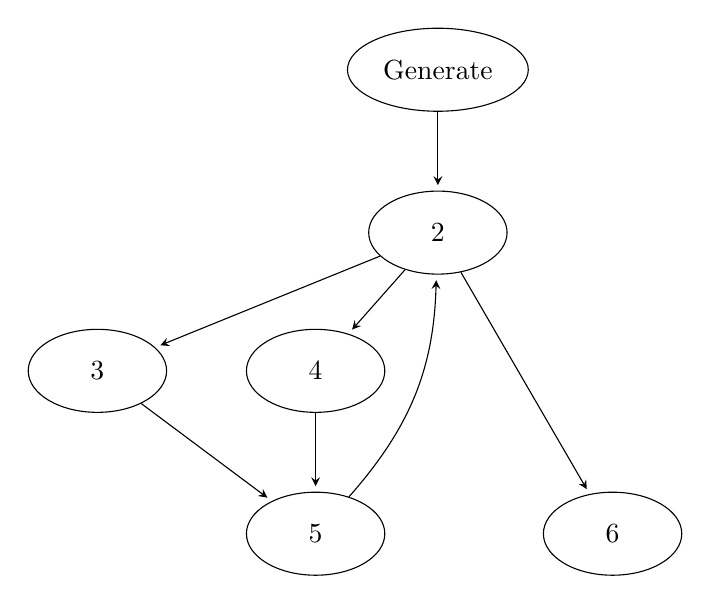
\begin{tikzpicture}[%
    ->,
    shorten >=2pt,
    >=stealth,
    node distance=1cm,
    noname/.style={%
      ellipse,
      minimum width=5em,
      minimum height=3em,
      draw
    }
  ]
    \node[noname] (1)                                             {Generate};
    \node[noname] (2) [below=of 1]                                {2};
    \node[noname] (4) [node distance=1cm and 3mm,below left=of 2] {4};
    \node[noname] (3) [left=of 4]                                 {3};
    \node[noname] (5) [below=of 4]                                {5};
    \node[noname] (6) [node distance=2cm,right=of 5]              {6};

    \path (1) edge                   node {} (2)
          (2) edge                   node {} (3)
          (2) edge                   node {} (4)
          (2) edge                   node {} (6)
          (3) edge                   node {} (5)
          (4) edge                   node {} (5)
          (5) edge [bend right=20pt] node {} (2);
  \end{tikzpicture}
\end{document}